\subsection{Earth-Sun system}

\subsubsection{Stability}

\begin{figure}[H]
    \centering
    \begin{subfigure}{0.5\textwidth}
        \centering
        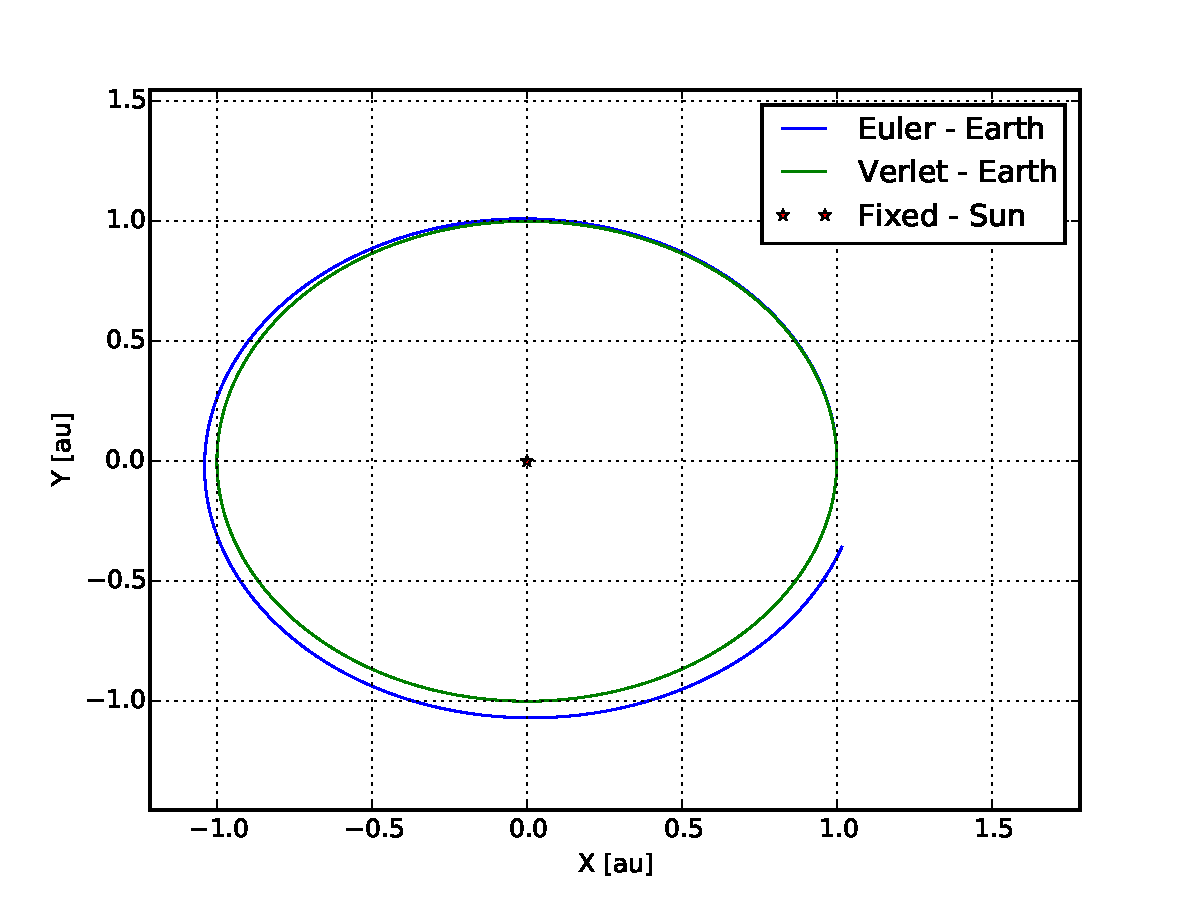
\includegraphics[width=\linewidth]{result/bilder/earth-sun.pdf}
    	\caption{}
    \end{subfigure}%
    ~ 
    \begin{subfigure}{0.5\textwidth}
        \centering
        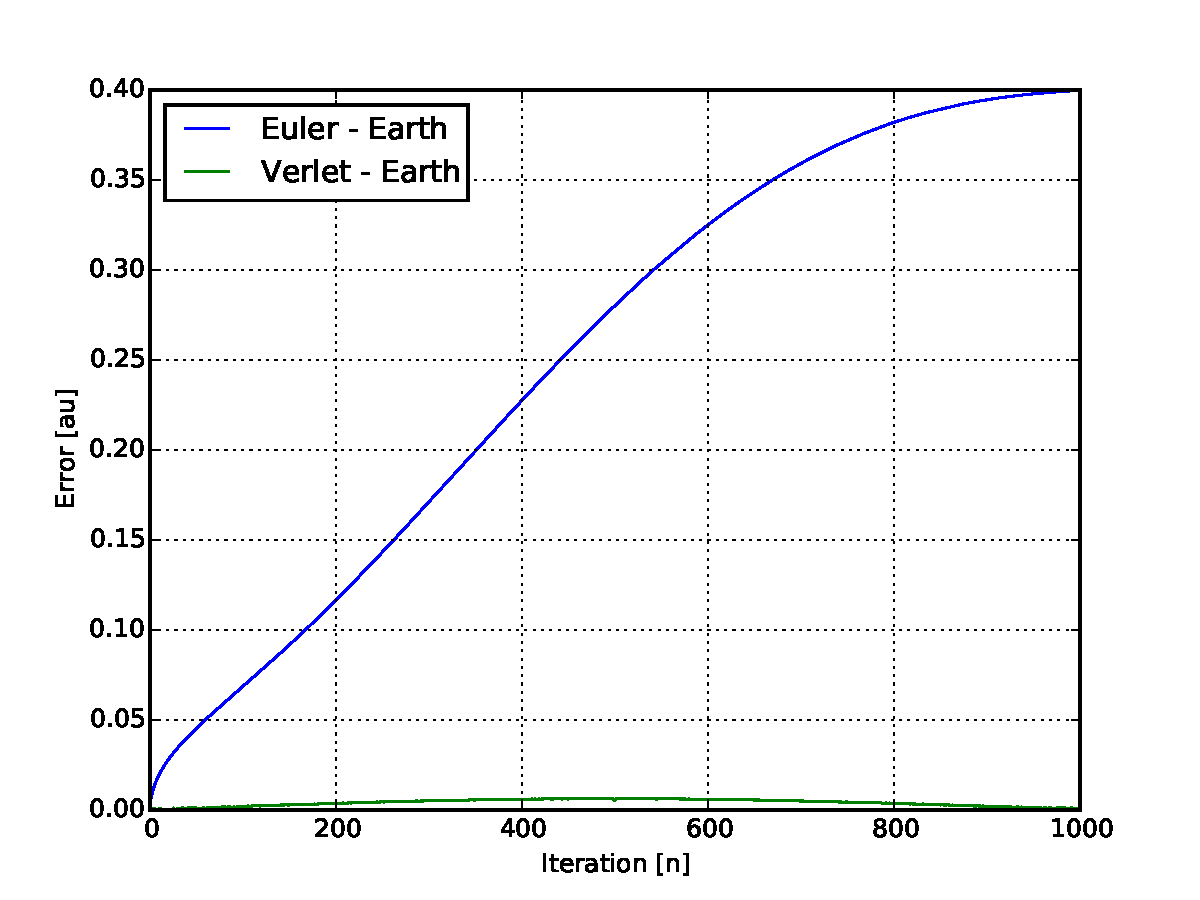
\includegraphics[width=\linewidth]{result/bilder/earth-sun-error.pdf}
        \caption{}
    \end{subfigure}
    \caption{a) show the orbit of earth around the sound. The intial velocity is set to $2\pi$ in y direction and the start position to 1 au in x direction. b) shows how the error behaves. The intial values should give a perfect circular motion. So the error is calculated by $r_i - r_{0}$. It is clear that Verlet-Velocity method is superior. This simulation was with 1000 points with the end time of 1 year. Both simulations was produced by \href{https://github.com/erikfsk/Project-3/blob/master/Project3/3a/plot_earth_sun.py}{\textcolor{blue}{plot\_earth\_sun.py}}}
    \label{fig:earth-sun}
\end{figure}

\todo{write about this tabular}
\begin{tabular}{|c|c|c|c|c|c|}
	\hline 
	n & Forward-Euler & Verlet-Velocity &  fastest & $\frac{slowest}{fastest}$\\ 
	\hline
	10 & 0.000136 & 0.000148 & Euler &   1.08823529412   \\ 
	\hline 
	100 & 0.000208 & 0.000179 & Verlet &   1.16201117318   \\ 
	\hline 
	1000 & 0.000392 & 0.000389 & Verlet &  1.00771208226   \\ 
	\hline
	10000 & 0.002427 & 0.002426 & Verlet &   1.00041220115  \\ 
	\hline
	100000 & 0.022931 & 0.022293 & Verlet &   1.02861884897   \\ 
	\hline
	1000000 & 0.167022 & 0.175944 & Euler &   1.05341811258  \\ 
	\hline
	10000000 & 1.58721 & 1.52666 & Verlet &   1.03966174525  \\ 
	\hline
	100000000 & 15.1786 & 15.1176 & Verlet &   1.00403503202  \\ 
	\hline
\end{tabular}



\subsubsection{Conserved quantities}


\begin{figure}[H]
    \centering
    \begin{subfigure}{0.5\textwidth}
        \centering
        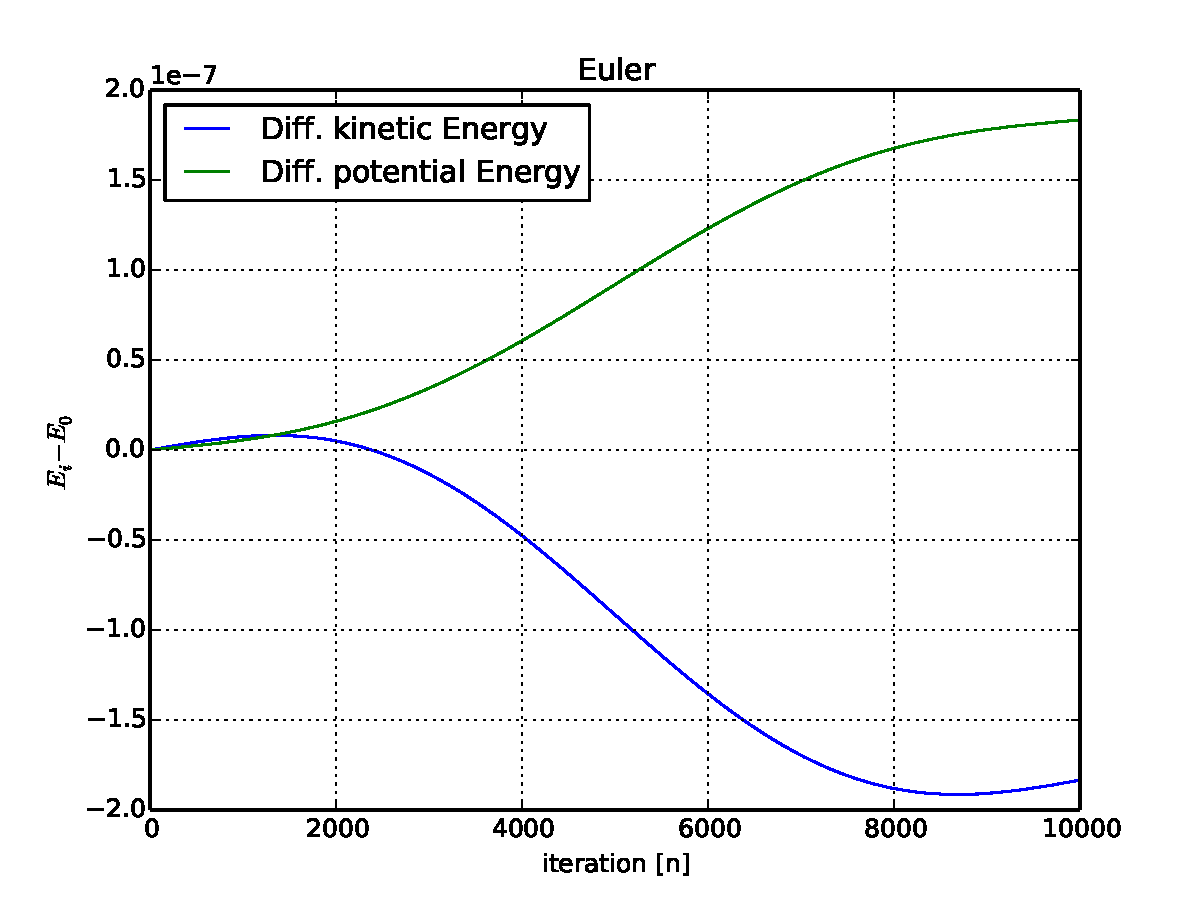
\includegraphics[width=\linewidth]{result/bilder/kin-pot-euler.pdf}
    	\caption{}
    \end{subfigure}%
    ~ 
    \begin{subfigure}{0.5\textwidth}
        \centering
        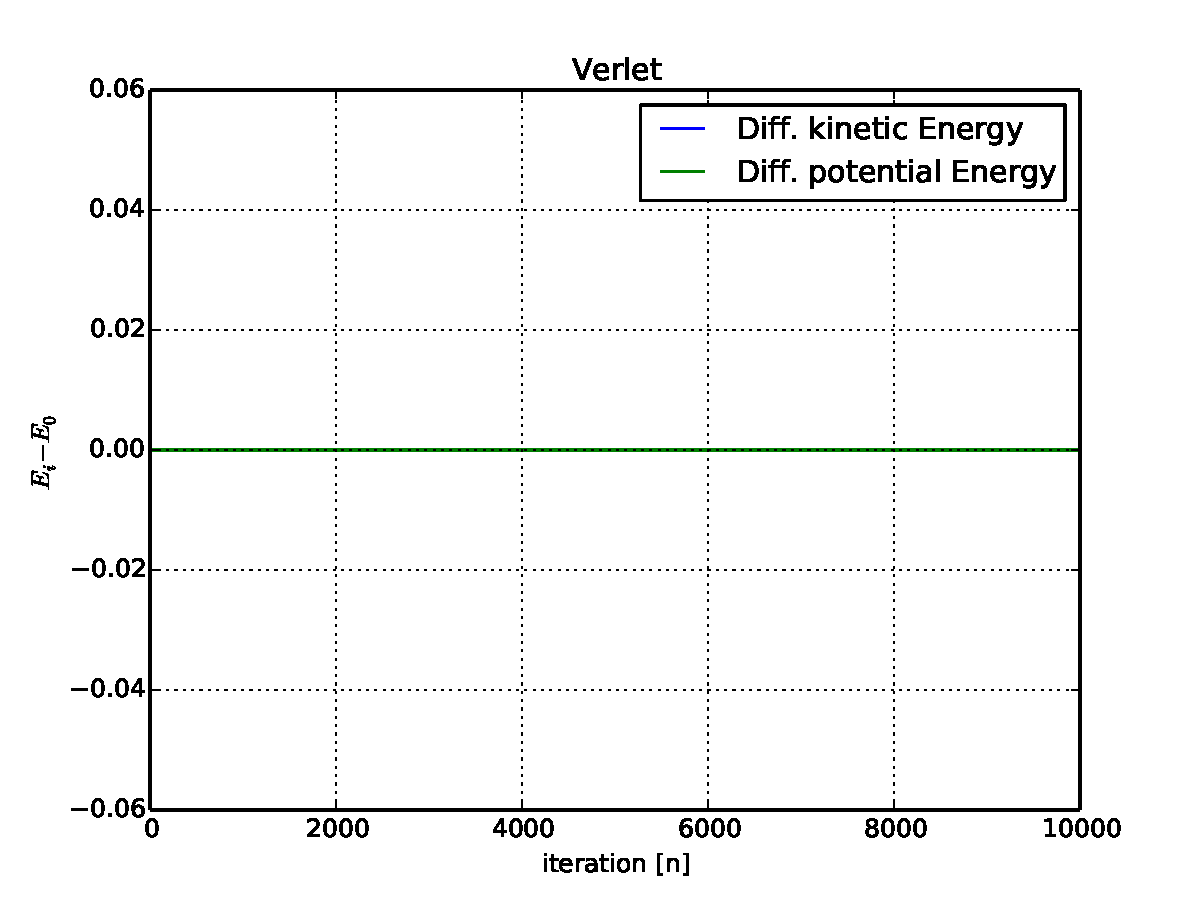
\includegraphics[width=\linewidth]{result/bilder/kin-pot-verlet.pdf}
        \caption{}
    \end{subfigure}
    \caption{\href{https://github.com/erikfsk/Project-3/blob/master/Project3/3a/plot_earth_sun.py}{\textcolor{blue}{plot\_earth\_sun.py}}}
    \label{fig:conserved-energy}
\end{figure}
\todo{write about this figure}


\begin{figure}[H]
    \centering
    \begin{subfigure}{0.5\textwidth}
        \centering
        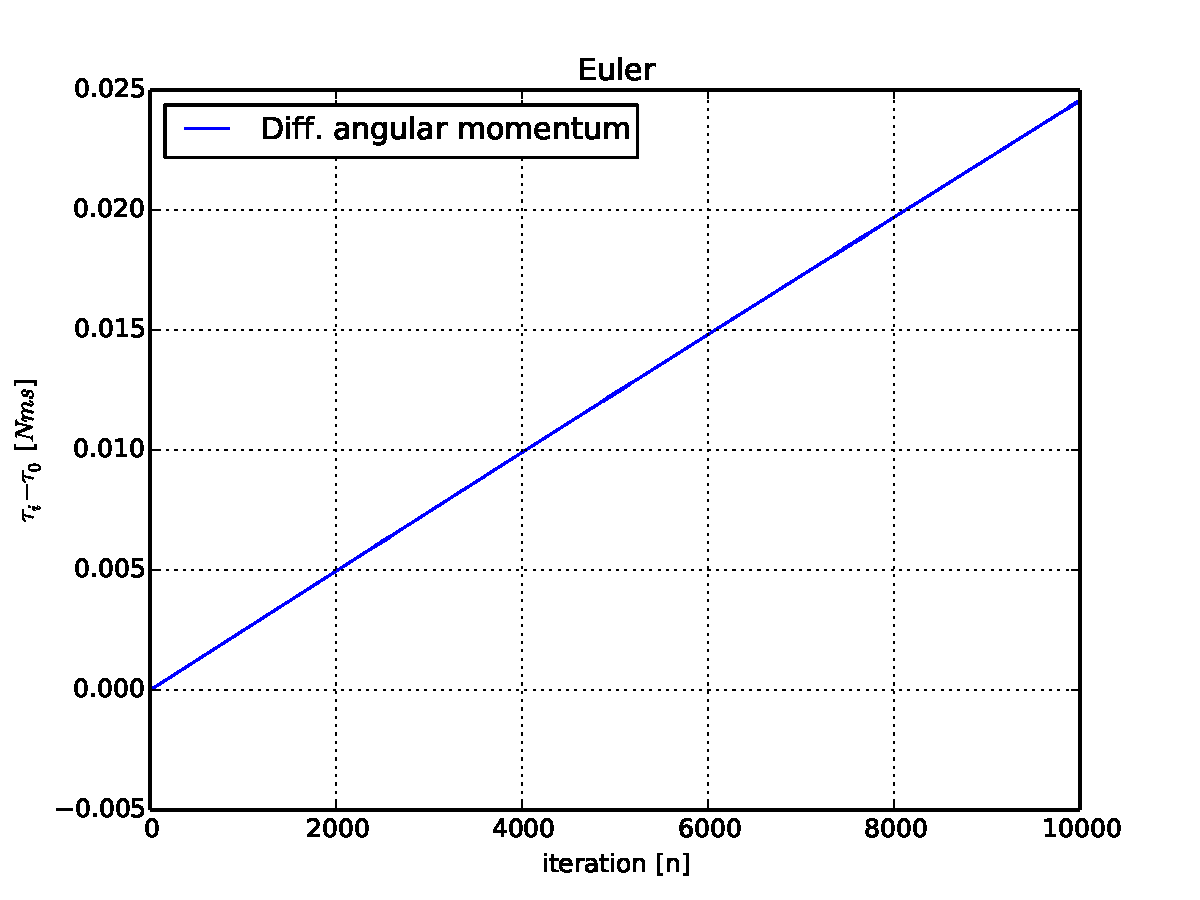
\includegraphics[width=\linewidth]{result/bilder/ang-momentum-euler.pdf}
    	\caption{}
    \end{subfigure}%
    ~ 
    \begin{subfigure}{0.5\textwidth}
        \centering
        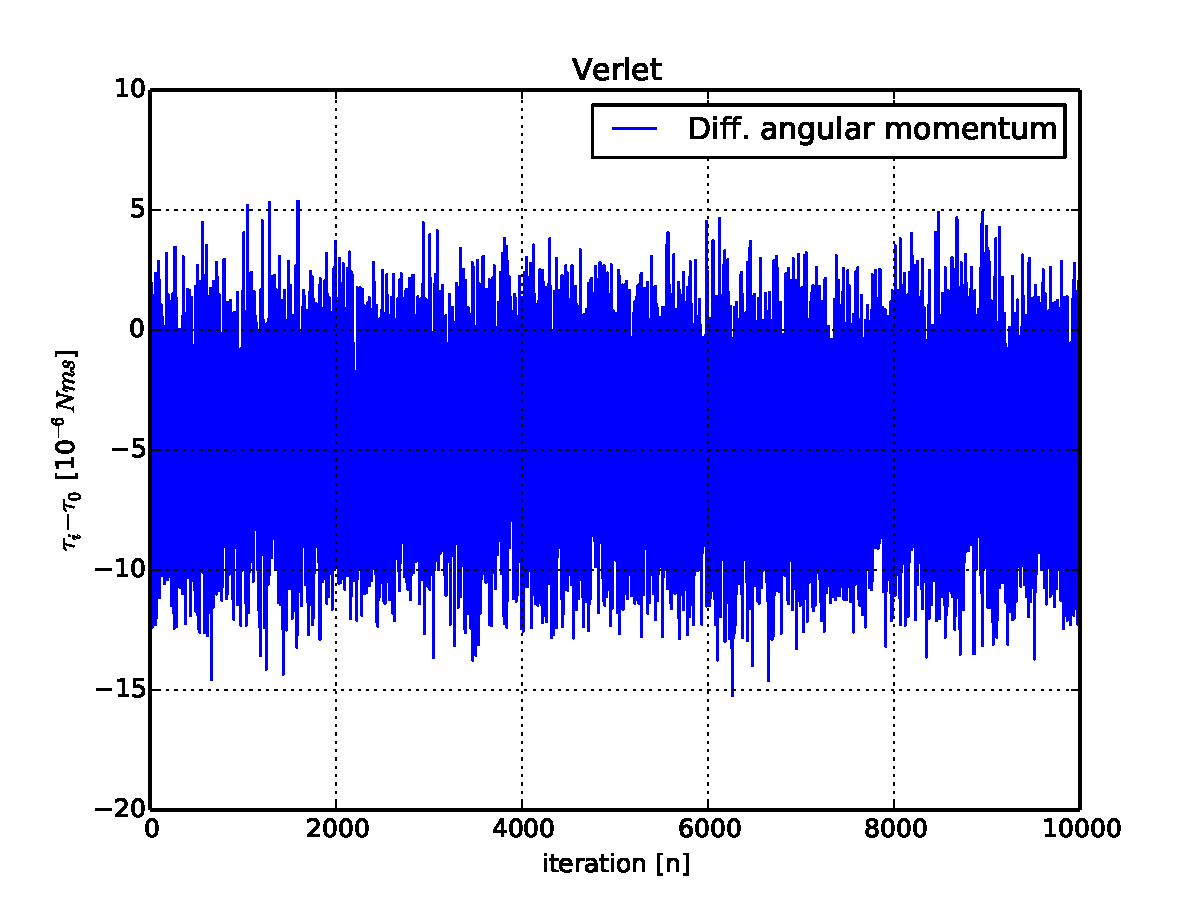
\includegraphics[width=\linewidth]{result/bilder/ang-momentum-verlet.pdf}
        \caption{}
    \end{subfigure}
    \caption{\href{https://github.com/erikfsk/Project-3/blob/master/Project3/3a/plot_earth_sun.py}{\textcolor{blue}{plot\_earth\_sun.py}}}
    \label{fig:conserved-ang}
\end{figure}
\todo{write about this figure}




\begin{figure}[H]
    \centering
    \begin{subfigure}{0.5\textwidth}
        \centering
        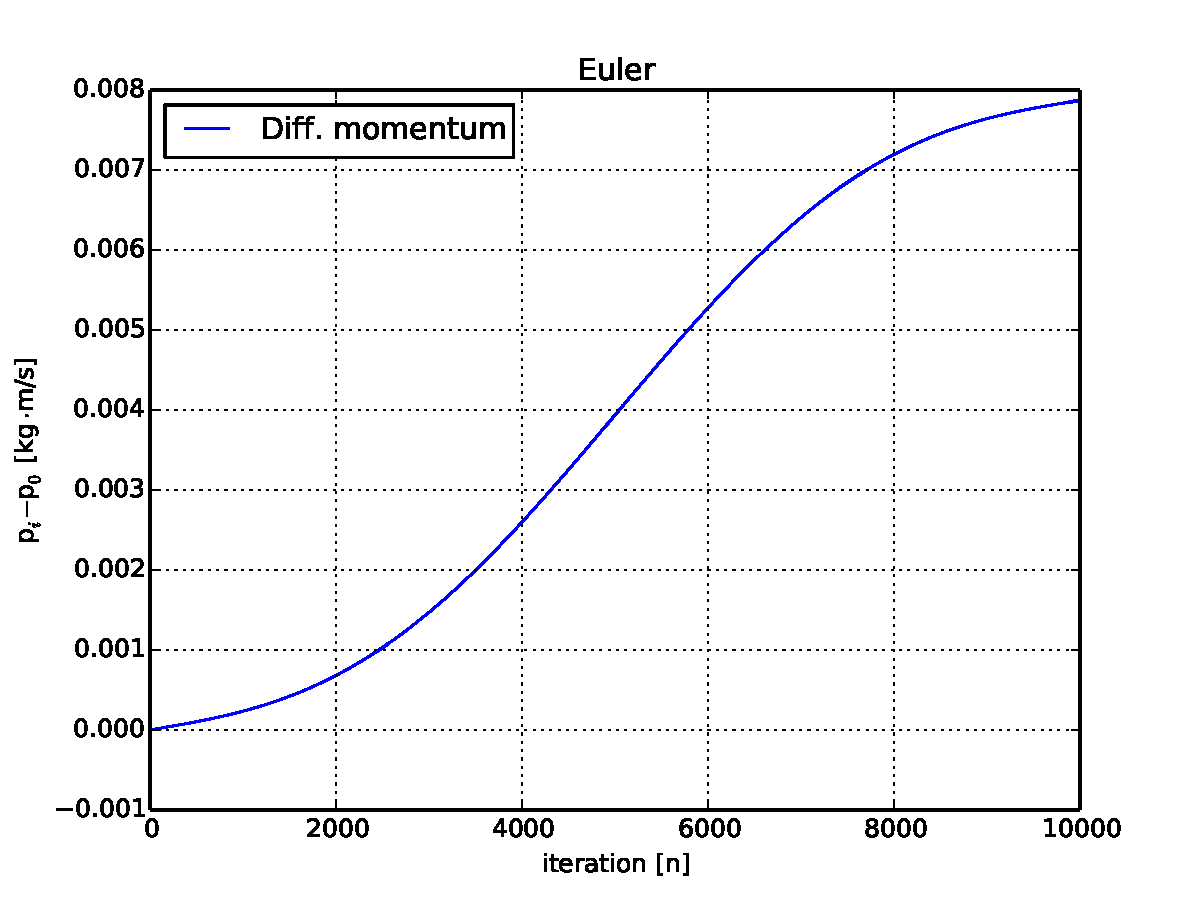
\includegraphics[width=\linewidth]{result/bilder/momentum-euler.pdf}
    	\caption{}
    \end{subfigure}%
    ~ 
    \begin{subfigure}{0.5\textwidth}
        \centering
        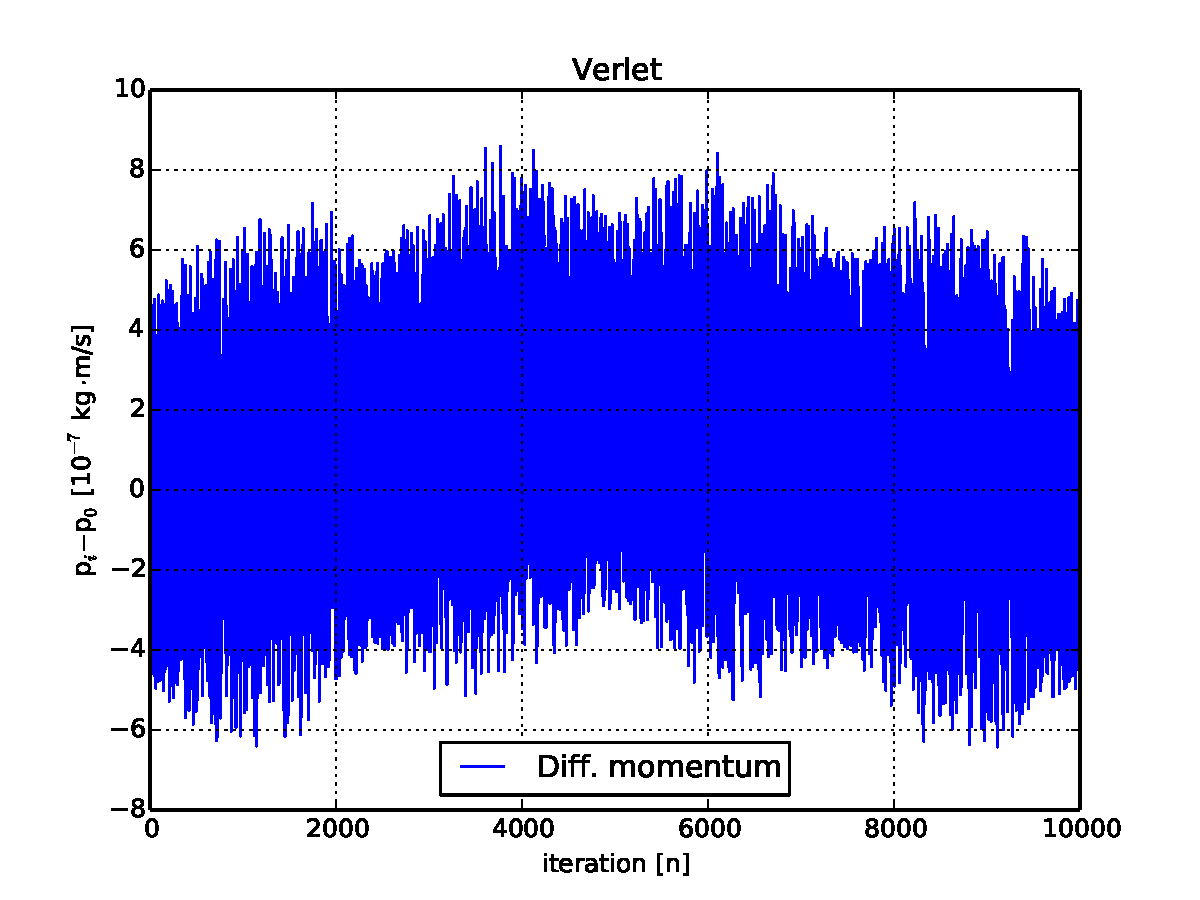
\includegraphics[width=\linewidth]{result/bilder/momentum-verlet.pdf}
        \caption{}
    \end{subfigure}
    \caption{\href{https://github.com/erikfsk/Project-3/blob/master/Project3/3a/plot_earth_sun.py}{\textcolor{blue}{plot\_earth\_sun.py}}}
    \label{fig:conserved-momentum}
\end{figure}
\todo{write about this figure}

















\subsubsection{Escape velocity}


\begin{figure}[H]
    \centering
    \begin{subfigure}{0.5\textwidth}
        \centering
        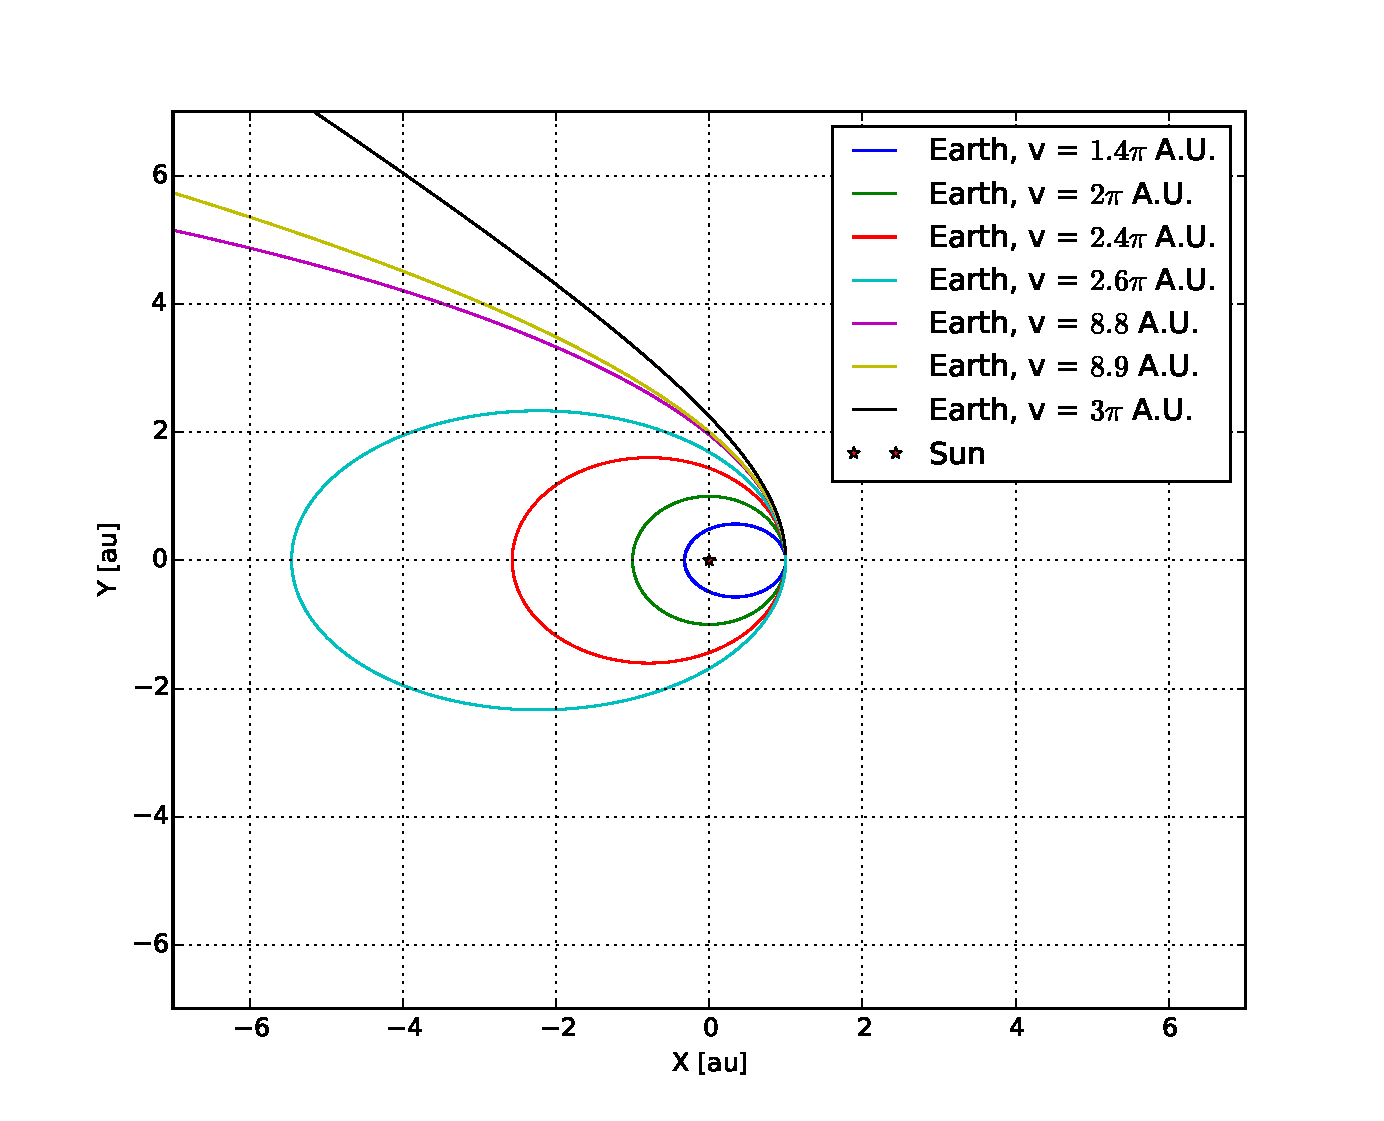
\includegraphics[width=\linewidth]{result/bilder/escape-velocity.pdf}
    	\caption{}
    \end{subfigure}%
    ~ 
    \begin{subfigure}{0.5\textwidth}
        \centering
        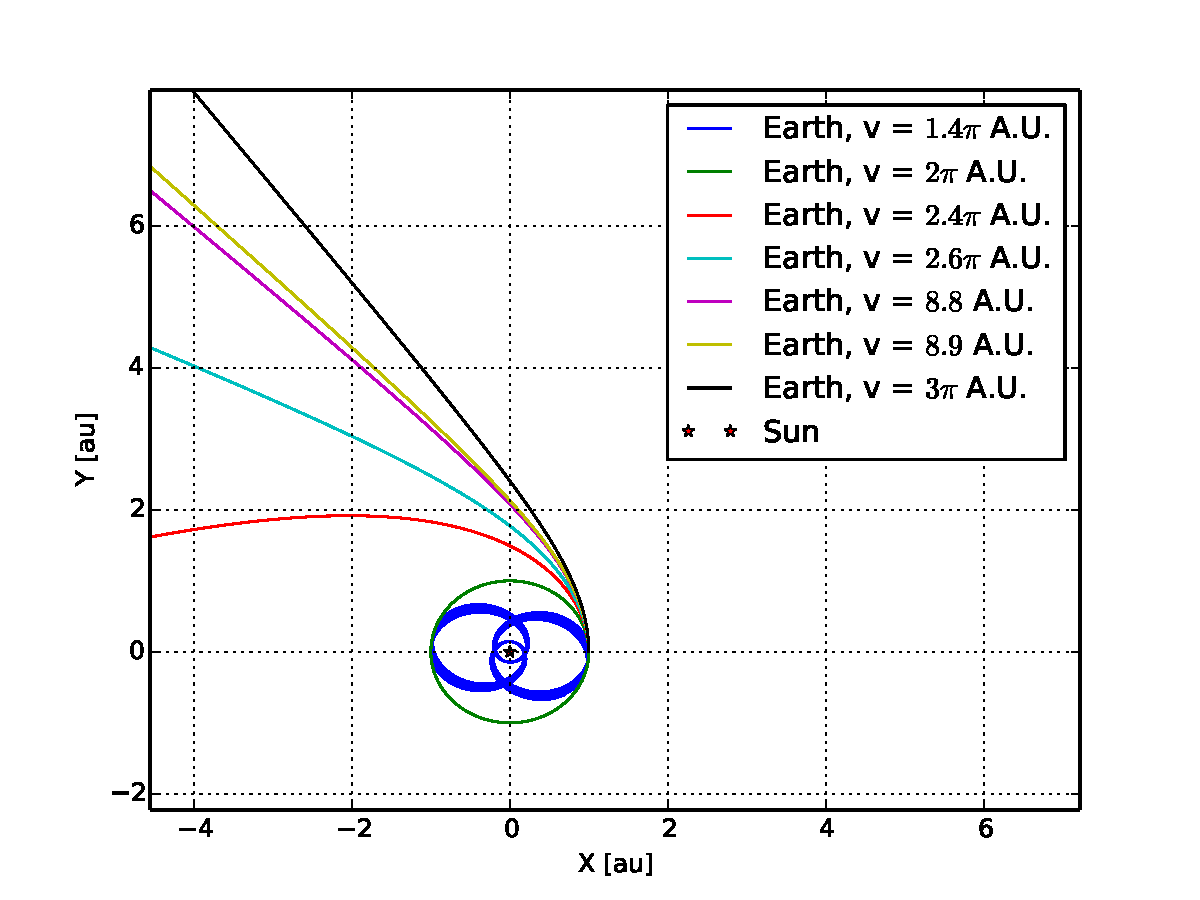
\includegraphics[width=\linewidth]{result/bilder/escape-velocity-r25.pdf}
        \caption{}
    \end{subfigure}
    \caption{\href{https://github.com/erikfsk/Project-3/blob/master/Project3/3a/plot_earth_sun.py}{\textcolor{blue}{plot\_earth\_sun.py}}}
    \label{fig:escape-velocity-low}
\end{figure}
\todo{write about this figure}



\begin{figure}[H]
    \centering
    \begin{subfigure}{0.5\textwidth}
        \centering
        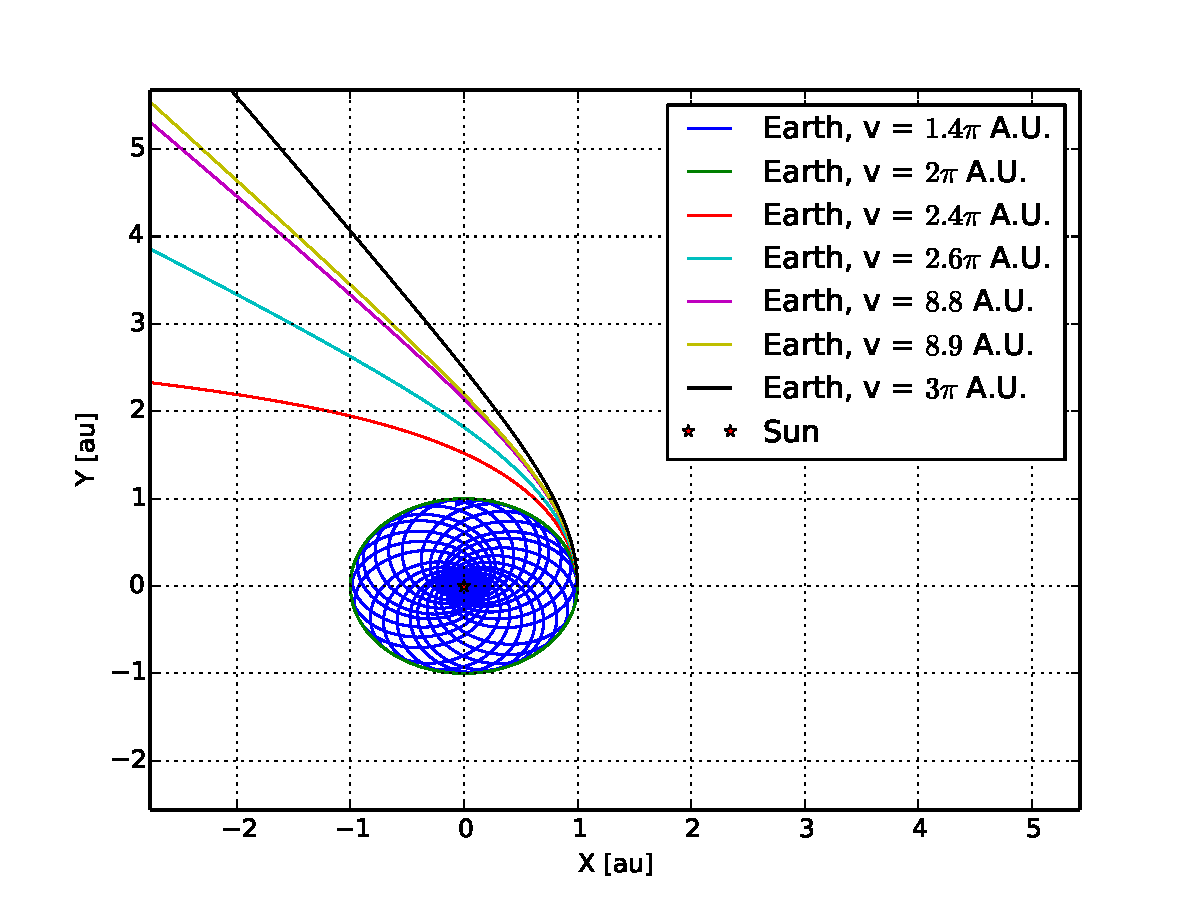
\includegraphics[width=\linewidth]{result/bilder/escape-velocity-r275.pdf}
    	\caption{}
    \end{subfigure}%
    ~ 
    \begin{subfigure}{0.5\textwidth}
        \centering
        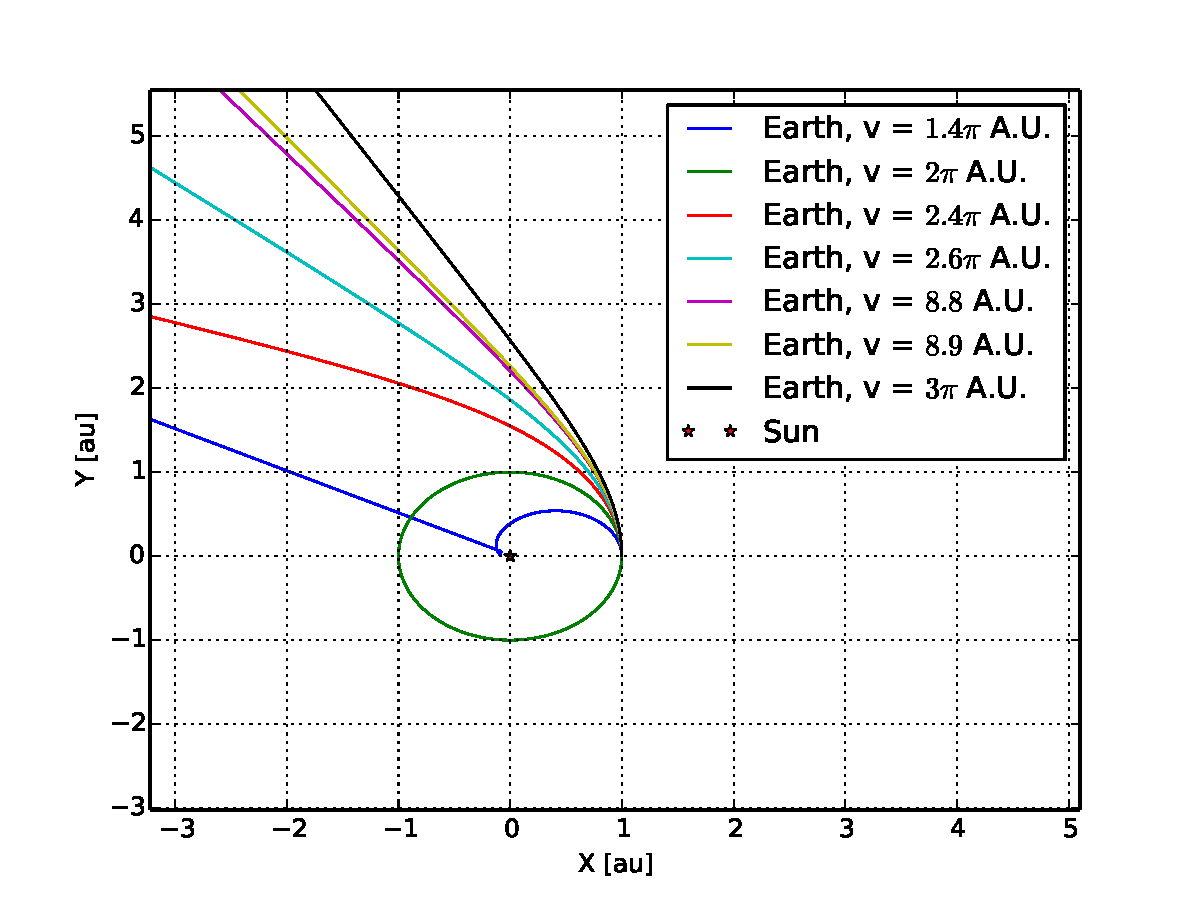
\includegraphics[width=\linewidth]{result/bilder/escape-velocity-r3.pdf}
        \caption{}
    \end{subfigure}
    \caption{\href{https://github.com/erikfsk/Project-3/blob/master/Project3/3a/plot_earth_sun.py}{\textcolor{blue}{plot\_earth\_sun.py}}}
    \label{fig:escape-velocity-high}
\end{figure}
\todo{write about this figure}

%\subsubsubsection{$r = 1$ A.U. and dependent on $r^2$}

%\subsubsubsubsection{Trial and error answer}

%\subsubsubsubsection{Numerical answer}


%\subsubsubsection{Varying dependency of radius}



\subsection{Three body system}

\subsubsection{Fixed mass for jupitur}


\subsubsection{Varying mass for jupitur}




\subsection{Solar system}


\subsubsection{Three planets and all moving}


\subsubsection{Solar system all moving}





\subsection{The perihelion precession of Mercury}

\subsubsection{missing this part}